\section{Фильтрация биржевых данных}
\subsection{Исходные данные}
Для примера я скачал данные о курсе акций компании SBER в период в первого апреля 2023 года по первое апреля 2024 года 
с промежутком в 1 день. 

Исходный график курса акций представлен на рисунке \ref{fig:source_quotes_\num}. 


\def\num{1}
\def\T{1} 

\begin{figure}[ht!]
    \centering
    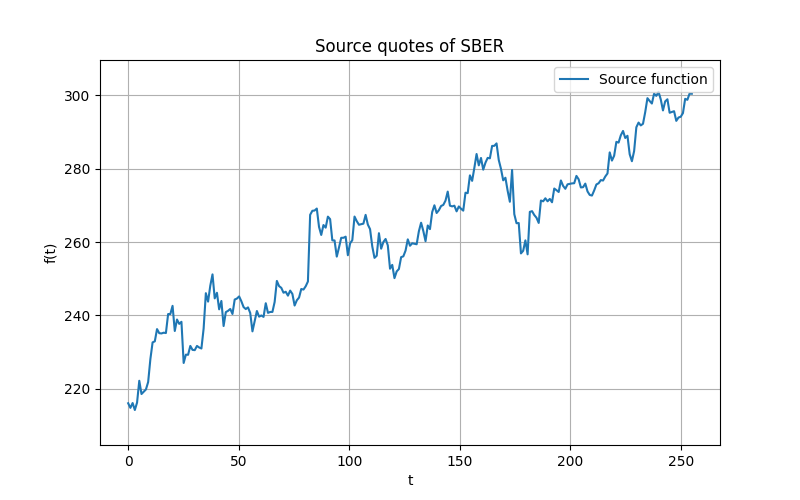
\includegraphics[width=\textwidth]{../results/third/\num/source_quotes}
    \caption{Исходные данные}
    \label{fig:source_quotes_\num}
\end{figure}

\subsection{Фильтрация данных}

Для фильтрации данных использовался фильтр первого порядка с параметром $T = \T$.
Данный параметр соответствует периоду сглаживания в 1 день.

Отфильтрованный график курса акций вместе с начальным представлены на рисунке \ref{fig:quotes_cmp_\num}.
\begin{figure}[ht!]
    \centering
    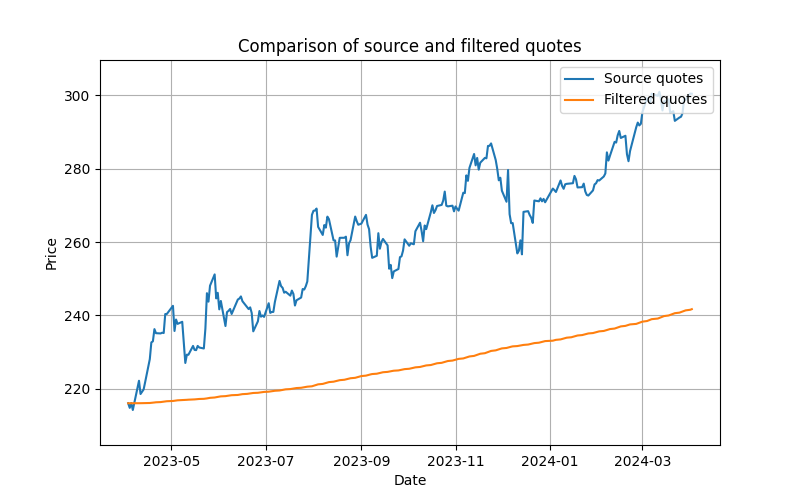
\includegraphics[width=\textwidth]{../results/third/\num/quotes_cmp}
    \caption{Отфильтрованные данные ($T = \T$)}
    \label{fig:quotes_cmp_\num}
\end{figure}

\def\num{2}
\def\T{7}
Теперь посмотрим на фильтр, который даст фильтрацию в 7 дней, ему соответствует параметр $T = \T$.

Для фильтрации данных использовался фильтр первого порядка с параметром $T = \T$.

Отфильтрованный график курса акций вместе с начальным представлены на рисунке \ref{fig:quotes_cmp_\num}.
\begin{figure}[ht!]
    \centering
    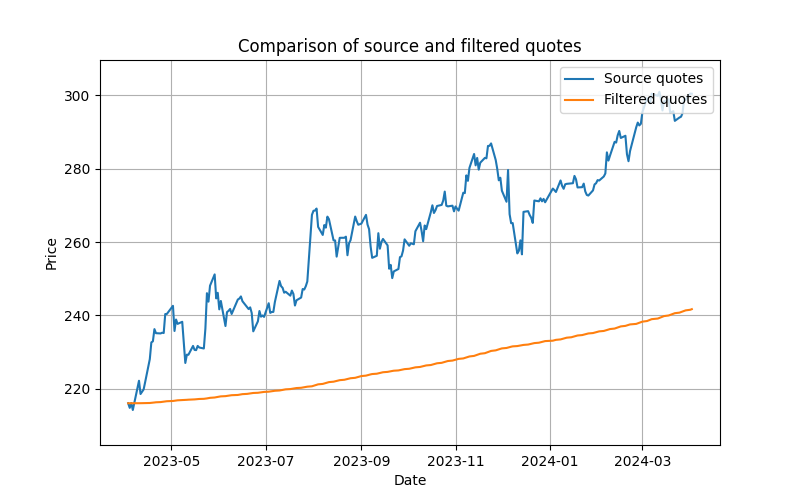
\includegraphics[width=\textwidth]{../results/third/\num/quotes_cmp}
    \caption{Отфильтрованные данные ($T = \T$)}
    \label{fig:quotes_cmp_\num}
\end{figure}

В данном случае фильтрация уже заметна. Видно, что график стал более гладким,
на нем убраны некоторые колебания в пределах одной недели, которые были на исходном графике. 

\FloatBarrier
Рассмотрим также другие значения $T$: 

\def\num{3}
\def\T{30}

\begin{figure}[ht!]
    \centering
    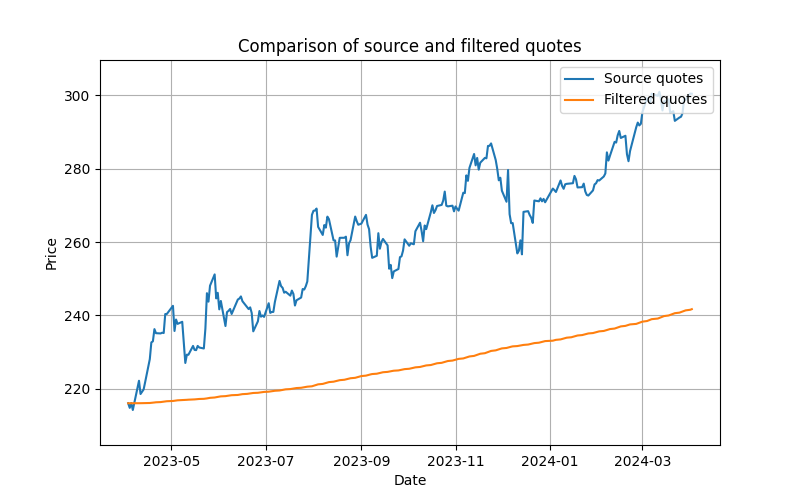
\includegraphics[width=\textwidth]{../results/third/\num/quotes_cmp}
    \caption{Отфильтрованные данные ($T = \T$)}
    \label{fig:quotes_cmp_\num}
\end{figure}

\def\num{4}
\def\T{90}

\begin{figure}[ht!]
    \centering
    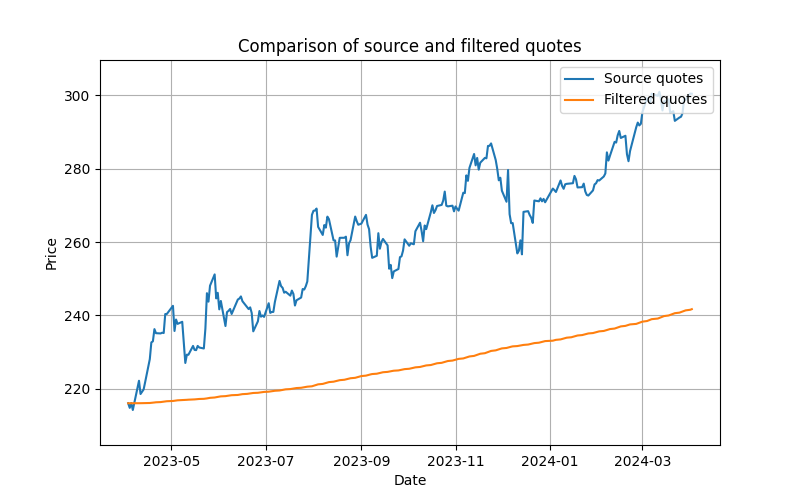
\includegraphics[width=\textwidth]{../results/third/\num/quotes_cmp}
    \caption{Отфильтрованные данные ($T = \T$)}
    \label{fig:quotes_cmp_\num}
\end{figure}


\def\num{5}
\def\T{356}

\begin{figure}[ht!]
    \centering
    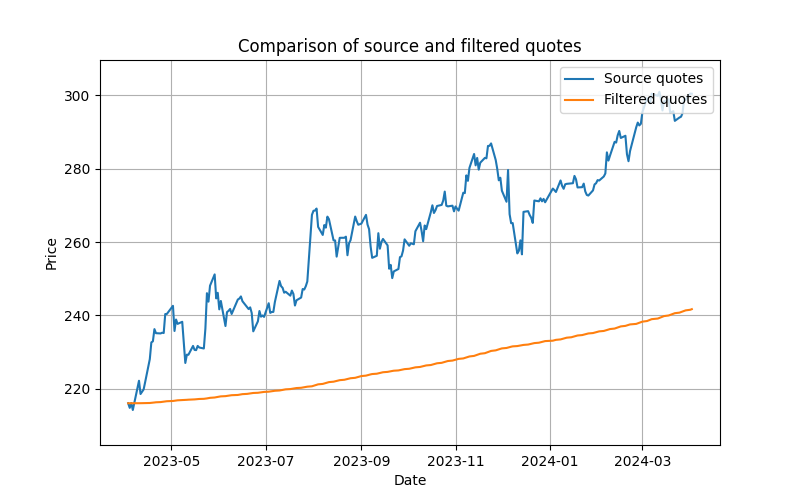
\includegraphics[width=\textwidth]{../results/third/\num/quotes_cmp}
    \caption{Отфильтрованные данные ($T = \T$)}
    \label{fig:quotes_cmp_\num}
\end{figure}

\FloatBarrier
\subsection{Выводы}
Видно, что при увеличении параметра $T$ график становится все более гладким, что и ожидается от фильтрации. 
Значения $T$ соответствуют периоду, колебания меньше которого будут подавляться. При значении $T = 1$ фильтрации 
практически не произошло, это связано с тем, что исходные данные и так не содержат колебаний в пределах одного дня.

Также видно, что при больших значениях $T$ график начинает сильно отличаться от исходного, что будет 
критично в случае фильтрации реальных данных. Это связано с тем, что я работаю с относительно небольшой выборкой данных (всего 255 точек, то есть дней в году, которые работала биржа). 
Более большой временной промежуток мне скачать не удалось. 

